% This work is licensed under the Creative Commons Attribution-NonCommercial 4.0 International License.
% To view a copy of this license, visit http://creativecommons.org/licenses/by-nc/4.0/
% or send a letter to Creative Commons, PO Box 1866, Mountain View, CA 94042, USA.

% !TEX TS-program = xelatex

\documentclass[../Main/chem371-notes.tex]{subfiles}

\setcounter{chapter}{1}
\begin{document}

\chapter{The Born--Oppenheimer Approximation and Potential Energy Surfaces}

(updated \today)

The previous chapter introduced the Schr\"{o}dinger equation and the molecular Hamiltonian.
At this point, we are going to examine an important approximation that allows us break down the complexity of the  Schr\"{o}dinger equation for molecules by separating the motion of electrons and nuclei.
We will also formalize the concept of potential energy surface.

\section{The Born--Oppenheimer or fixed nuclei approximation}
One important simplification of the Schr\"{o}dinger equation is to separate the motion of the electrons and the nuclei.
This approach is justified by the fact that the mass of a nucleus is at least 1836 times larger than that of an electron.
A good analogy is that of flies (electrons) that move around cows (nuclei). The motion of the flies does not perturb the cows, but if a cow moves then all the flies will rapidly readjust their motion to follow the cow.
\mfigure{
\centering{
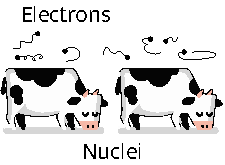
\includegraphics[width=1.75in]{img/born-oppenheimer-cow-fly.pdf}
}
\captionof{figure}{The fly/cow analogy of the Born--Oppenheimer approximation.}
}

In the fixed nuclei approximation, also known as \emph{Born--Oppenheimer approximation}, we separate the wave function of electron and nuclei in the following way
\begin{iequation}
\Psi(\mathbf{r}, \mathbf{R})
\approx \Psi_{\mathbf{R}}^\mathrm{el}(\mathbf{r}) \Psi^\mathrm{nuc}(\mathbf{R})
\end{iequation}
where to keep these expression compact we have indicated the coordinates of all electrons and nuclei with a single variable, that is, $\mathbf{r} = (\mathbf{r}_1, \mathbf{r}_2, \ldots)$ and $\mathbf{R} = (\mathbf{R}_1, \mathbf{R}_2, \ldots)$.

This equation says that the total wave function can be written as a wave function for the electrons ($\Psi^\mathrm{el}$) times the wave function for the nuclei ($\Psi^\mathrm{nuc}$).
Note that $\Psi^\mathrm{nuc}$ only depends on the coordinate of the nuclei (nuclei are like the cows, they can almost completely ignore the exact position of the electrons).
In contrast, the electron wave function depends both on the coordinate of the nuclei and the electrons.
However, the way you should think of this as a function of the electron coordinates that depends \emph{parametrically} on the position of the nuclei $ \mathbf{R}_1,  \mathbf{R}_2,\ldots$ (in our analogy, the electrons are like the flies, their position depends significantly on the position of the cows).

When we assume the Born--Oppenheimer approximation, the Hamiltonian for the electrons takes a simpler form
\begin{equation}
\hat{H}^\mathrm{el} = \hat{T}_\mathrm{e} + \hat{V}_\mathrm{ee} + \hat{V}_\mathrm{en} + V_\mathrm{nn}
\end{equation}
The first term in this expression is just the kinetic energy of the electrons. The second term accounts for the electron-electron repulsion energy. The third term is the electron-nuclear attraction (attractive force acting on the electron). In this approximation, the last term is just a constant, which accounts for the nuclear-nuclear repulsion energy.\mnote{
The nuclear-nuclear repulsion energy is given by
\begin{equation}
V_\mathrm{nn} = \frac{1}{4\pi \epsilon_0}  \sum_{i < j}^{\mathrm{nuclei}} \frac{q_i q_j}{R_{ij}}
\end{equation}
}

The wave functions for the electronic in the BO approximation satisfies the following Schr\"{o}dinger equation
\begin{equation}
\hat{H}^\mathrm{el}\Psi_{\mathbf{R}}^\mathrm{el}(\mathbf{r}) =
E(\mathbf{R})
\Psi_{\mathbf{R}}^\mathrm{el}(\mathbf{r})
\end{equation}
which yields the potential energy $E(\mathbf{R})$, a quantity that depends on the position of the nuclei.

The  potential energy $E(\mathbf{R})$ is the central quantity that computational chemists aim to obtain when doing a quantum chemistry computation.
Once you have $E(\mathbf{R})$ you can determine the structure of a molecule, the way it reacts.
If we then solve the Schr\"{o}dinger equation for the nuclei using the potential energy $E(\mathbf{R})$, we can even obtain information about the vibrational (IR) spectroscopy of molecules. 
We will come back to this topic in a later chapter.

\section{The potential energy surface of diatomic molecules}
\mfigure{
\centering{
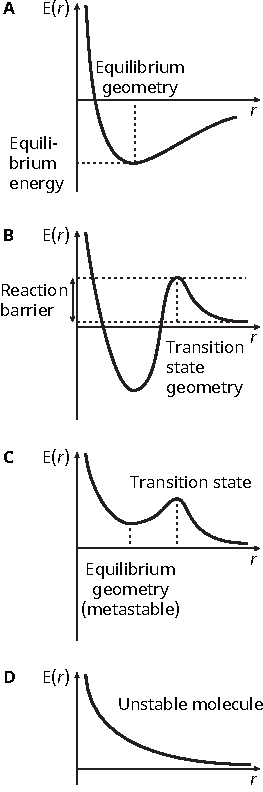
\includegraphics[width=1.75in]{img/diatomic.pdf}
}
\captionof{figure}{The potential energy surface for a diatomic molecule. \textbf{A} and \textbf{B} show typical stable diatomic molecule. \textbf{C} and \textbf{D} show the case of a metastable molecule (stable only for a finite time) and an unstable molecule, respectively.}
\label{fig:diatomic}
}

The Born--Oppenheimer approximation is fundamental to our understanding of chemistry and  it one that you are already very familiar with, even though you might have not realized it.
This approximation is implicitly assumed when you first learn about quantum mechanics in introductory chemistry courses.
Once we solve the Schr\"{o}dinger equation in the BO approximation, the energy of the electrons depends on the coordinates of the nuclei
\begin{equation}
E = E(\mathbf{R}_1,  \mathbf{R}_2,\ldots)
\end{equation}
This is why we can talk about a molecule having a certain energy at a given nuclear configuration.
The quantity $E(\mathbf{R}_1,  \mathbf{R}_2,\ldots)$ represents the potential felt by the nuclei due to the interaction with the electrons, and since it is a function of many variables it is commonly called the \emph{potential energy surface}.

Many of the concepts about the structure and energetics of molecules are derived from the properties of potential energy surface.
These include the notion of molecular equilibrium structure, equilibrium energy, transition states, and reaction barriers.

The potential energy surface for a diatomic molecule \ce{A-B} is easy to visualize, because the energy depends only on the bond distance $r$, that is, $E = E(r)$, and we call it a \emph{potential energy curve} (PEC).
Fig.~\ref{fig:diatomic} shows four potential energy surfaces for a diatomic molecule.
The top two plots show a stable \ce{AB} molecule.
In the first case (\textbf{A}), the reaction \ce{A + B} $\rightarrow$ {AB} is barrier-less and happens spontaneously.
The bond distance $r_e$ where the energy of AB is a minimum is the \emph{equilibrium geometry}, and the corresponding energy is the \emph{equilibrium energy}.
In the second case  (\textbf{B}),  the reaction \ce{A + B} $\rightarrow$ {AB} proceeds via a \emph{transition state} \ce{AB}* that has an energy higher than \ce{A + B}.
This reaction can happen only if A and B collide with enough energy to overcome the \emph{reaction barrier}.

Mathematically, both equilibrium geometries and transition states correspond to \emph{stationary points} $r^*$ on the potential energy curve, which are characterized by a zero first derivative with respect to $r$
\begin{equation}
\text{At a stationary point } r^*: \quad \left.\frac{d E(r)}{dr}\right|_{r = r^*} = 0
\end{equation}
What distinguishes an equilibrium geometry and a transition state is the \emph{curvature} of the potential energy curve at $r^*$.
For equilibrium geometries, the energy is a minimum and the curvature is positive, that is, the second derivative of the potential is positive
\begin{equation}
\text{At a minimum } r^*: \quad \left.\frac{d^2 E(r)}{dr^2}\right|_{r = r^*} > 0
\end{equation}
A transition state instead corresponds to a negative curvature or negative second derivative
\begin{equation}
\text{At a transistion state } r^*: \quad \left.\frac{d^2 E(r)}{dr^2}\right|_{r = r^*} < 0
\end{equation}

Plots \textbf{C} and \textbf{D} show two other scenarios in which the molecule AB is unstable.
When there is transition state (\textbf{C}), then we call a molecule \emph{metastable}, because it may be able to exist for a short amount of time before breaking down into A + B.
If there is no transition state (\textbf{D}), then the molecule AB is unstable and the two atoms will seek to be as far as possible.



\section{Potential energy surfaces of polyatomic molecules}

More general potential energy surfaces are more difficult to visualize because  $E(\mathbf{R}_1,  \mathbf{R}_2,\ldots)$ is a high-dimensional hypersurface.
For example, a molecule like \ce{H3CNO} has a potential energy surface that has 13 dimensions!

A much simpler case is that of a molecule with three atoms (ABC), which corresponds to a potential energy surface in four dimensions (this number comes from taking three coordinates for each atom $3 \times 3 = 9$ plus the energy, and subtracting 3 degrees of freedom for rotations and 3 for translations).
However, if we fix one of these three dimensions, for example, if we keep the angle A-B-C at 180\textdegree, then the resulting surface lives in only three dimensions and we can easily plot it.
In this case, we can represent the potential energy surface with a contour map, in a way similar to topographic maps, which have two dimensions, and the third dimension is indicated by contour lines.

Fig.~\ref{fig:abc} shows the contour map for a hypothetical \ce{A-B-C} system.
You can tell that there are two equilibrium structures. Of these two, the one that corresponds to small values of the BC bond distance is more stable, an it corresponds to the BC molecule weakly interacting with A (\ce{A\bond{...}B-C}).
The second minimum (a local minimum) corresponds to the molecule AB weakly interacting with C (\ce{A-B\bond{...}C}).
These two structures, are separated by a transition state \ce{A-B-C}.
These plots also show a the minimum energy reaction path that connects \ce{A + BC} to \ce{AB + C} and the corresponding energy potential.
To go from \ce{A\bond{...}B-C} to \ce{A-B\bond{...}C}, the molecule has to overcome a reaction barrier.
As you can see from the plot in \textbf{C}, the height of this barrier depends on the direction of the reaction.  

\mfigure{
\centering{
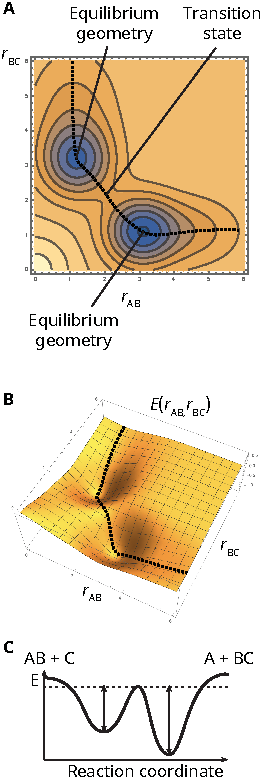
\includegraphics[width=1.75in]{img/abc.pdf}
}
\captionof{figure}{The potential energy surface for a linear triatomic molecule. \textbf{A} and \textbf{B} show the potential energy surface plotted using a contour plot and in 3D, respectively. A reaction path connecting \ce{A + BC} to \ce{AB + C} is shown, which goes through two local minima and one transition state. The energy profile for this reaction coordinate is shown in \textbf{C}.}
\label{fig:abc}
}

\end{document}